%% LaTeX-Beamer template for KIT design
%% by Erik Burger, Christian Hammer
%% title picture by Klaus Krogmann
%%
%% version 2.4
%%
%% mostly compatible to KIT corporate design v2.0
%% http://intranet.kit.edu/gestaltungsrichtlinien.php
%%
%% Problems, bugs and comments to
%% burger@kit.edu

%% Class options
%%   aspect ratio options: 
%%   -- 16:9 (default)
%%   -- 4:3
%%   language options: 
%%   -- en (default)
%%   -- de
%%   position of navigation bar:
%%   -- navbarinline (default): bottom of the white canvas
%%   -- navbarinfooter : more compressed variant inside the footer
%%   -- navbarside : side bar at the left of the white canvas
%%   -- navbaroff : none
%% example: \documentclass[16:9,de,navbarinfooter]{sdqbeamer}
\documentclass[16:9,en,navbarinfooter]{sdqbeamer}

%% \documentclass{sdqbeamer} 

%% TITLE PICTURE

% if a custom picture is to be used on the title page, copy it into the 'logos'
% directory, in the line below, replace 'myimage' with the 
% filename (without extension) and uncomment the following line
% (picture proportions: 63 : 20 for standard, 169 : 40 for wide
% *.eps format if you use latex+dvips+ps2pdf, 
% *.jpg/*.png/*.pdf if you use pdflatex)

% \titleimage{myimage}

%% GROUP LOGO 

% for a custom group logo, copy your file into the 'logos'
% directory, insert the filename in the line below and uncomment it

\grouplogo{irl-logo}

% (*.eps format if you use latex+dvips+ps2pdf,
% *.jpg/*.png/*.pdf if you use pdflatex)

%% GROUP NAME

% for groups other than SDQ, please insert in the line below and uncomment it
% \groupname{My group}

% the presentation starts here 

\author{Caspar Friedrich Maximilian Nagy}

%% Title (and possibly subtitle) of the thesis
\title{Solving Real-World Robot Manipulation Tasks with Deep Reinforcement Learning}
\subtitle{Box Pushing on a real Panda Robot}

% Bibliography 
\usepackage{dsfont}
%\usepackage{multimedia}
%\usepackage{media9}
\usepackage{booktabs}
\usepackage{longtable}
\usepackage{color}
\usepackage{array}
\usepackage{algorithm}
\usepackage{algpseudocode}
\usepackage{pgfplots}
% \pgfplotsset{compat=1.15}
 \usepgfplotslibrary{groupplots}
\usepackage{subcaption}
\usepackage{pdflscape}
\usepackage{diagbox}
\usepackage{multicol}
\DeclareUnicodeCharacter{2212}{−}
\usepgfplotslibrary{groupplots,dateplot}
\usetikzlibrary{patterns,shapes.arrows}
\pgfplotsset{compat=newest}
\usepackage[citestyle=authoryear,bibstyle=numeric,hyperref,backend=biber%,style=verbose
]{biblatex}
\addbibresource{presentation.bib}
\bibhang1em
\usepackage{listings}
\begin{document}

%title page
\KITtitleframe{}

%table of contents

\begin{frame}
\frametitle{Agenda}
\tableofcontents
\end{frame}

\section{Motion Primitive-Based (Re-)Planning Policy (MP3)}
\begin{frame}{Motion Primitive-Based (Re-)Planning Policy (MP3)}

\begin{columns}[t]
    \begin{column}{\textwidth}
        \begin{itemize}
            \item Idea: let agent choose parameters of trajectory generator instead of low-level actions
                \begin{itemize}
                    \item We use ProDMPs for their replanning-ability
                \end{itemize}
            \item Leads to smooth trajectories, correlated exploration
            \item Can use sparse, non-markovian rewards
            \item Blackbox and replanning variant
            \item Train on-policy using Trust Region Projection Layers (TRPL)
        \end{itemize}
    \end{column}
    %\movie[width=\linewidth]{MP3-Replan Boxpushing}{media/7dof_boxpushing_replan.mp4}
    \begin{column}{0.5\textwidth}
    \end{column}
\end{columns}
\vspace{1cm}
     We have impressive results with simulated environments, but how well do they work in the real world?
\end{frame}

\begin{frame}{Box Pushing}
\section{Box Pushing}

\begin{columns}[t]
    \begin{column}{0.5\textwidth}
        \begin{itemize}
            \item Goal: Use a finger to push a box to a target pose
                \begin{itemize}
                    \item Random start pose
                    \item Fixed target pose
                \end{itemize}
            \item Action space: 2D finger positions
            \item Observation:
                \begin{itemize}
                    \item Finger Position
                    \item Box Quaternion
                    \item Box Position
                \end{itemize}
        \end{itemize}
            \vspace{1em}
    \end{column}
    \begin{column}{0.5\textwidth}
        $$
        \begin{aligned}
    \text{Reward} &= \text{Final Euclidean Distance} \\
             &+  \text{Final Rotational Distance} \\
             &+  \mathds{1} \left\{\text{eucl. dist < 5cm and rot. dist < .5rad}\right\} \\
             &+  \max_t\  step(v_t) \\
             &+  \sum_t \left\Vert x_t - x_t^\text{clipped} \right\Vert \\
        \end{aligned}
        $$
    \end{column}
\end{columns}
\end{frame}

\begin{frame}{Box Pushing --- MuJoCo Simulation}
\begin{columns}
    \begin{column}{0.3\textwidth}
        \begin{itemize}
                \item The box has friction and mass as measured on the real box
                \item Finger has fixed height and orientation
                \item PD position control with randomized parameters to match Panda Kinematics
        \end{itemize}
    \end{column}
    \begin{column}{0.6\textwidth}
        \vspace{1cm}
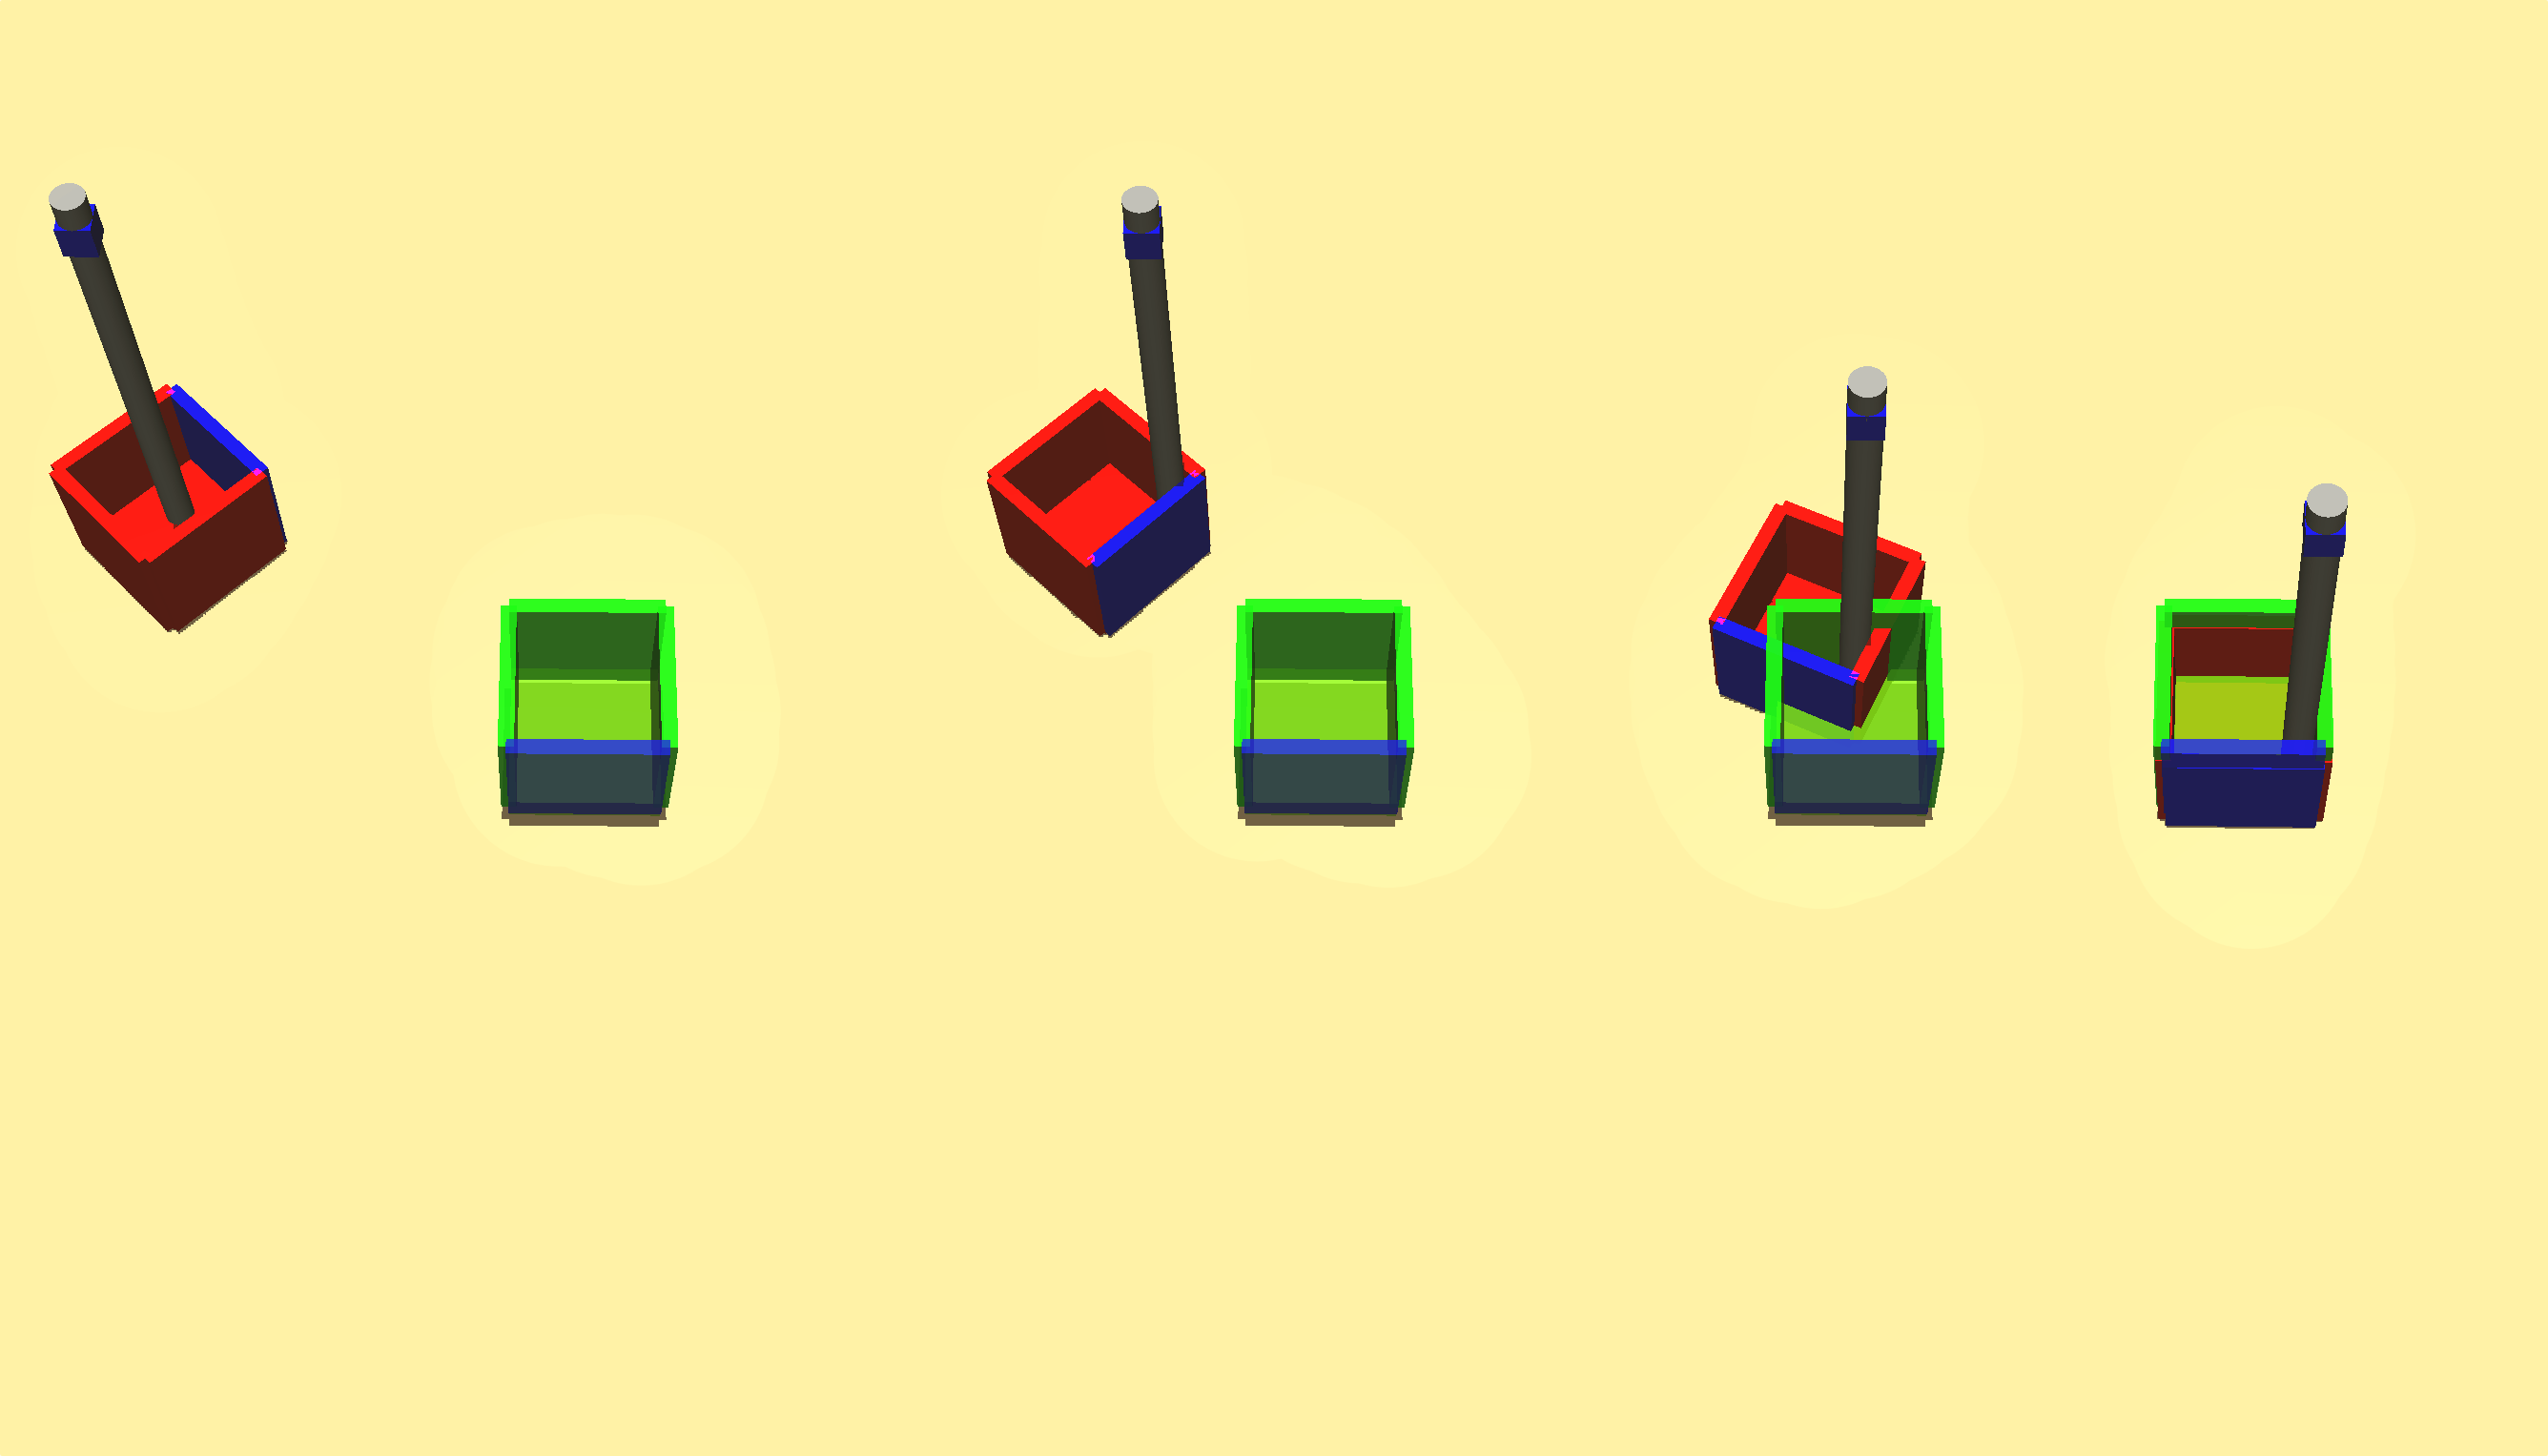
\includegraphics[width=\linewidth]{media/2dboxpushing}
    \end{column}
\end{columns}

\end{frame}

\begin{frame}{Box Pushing --- Lab Setup}
\center
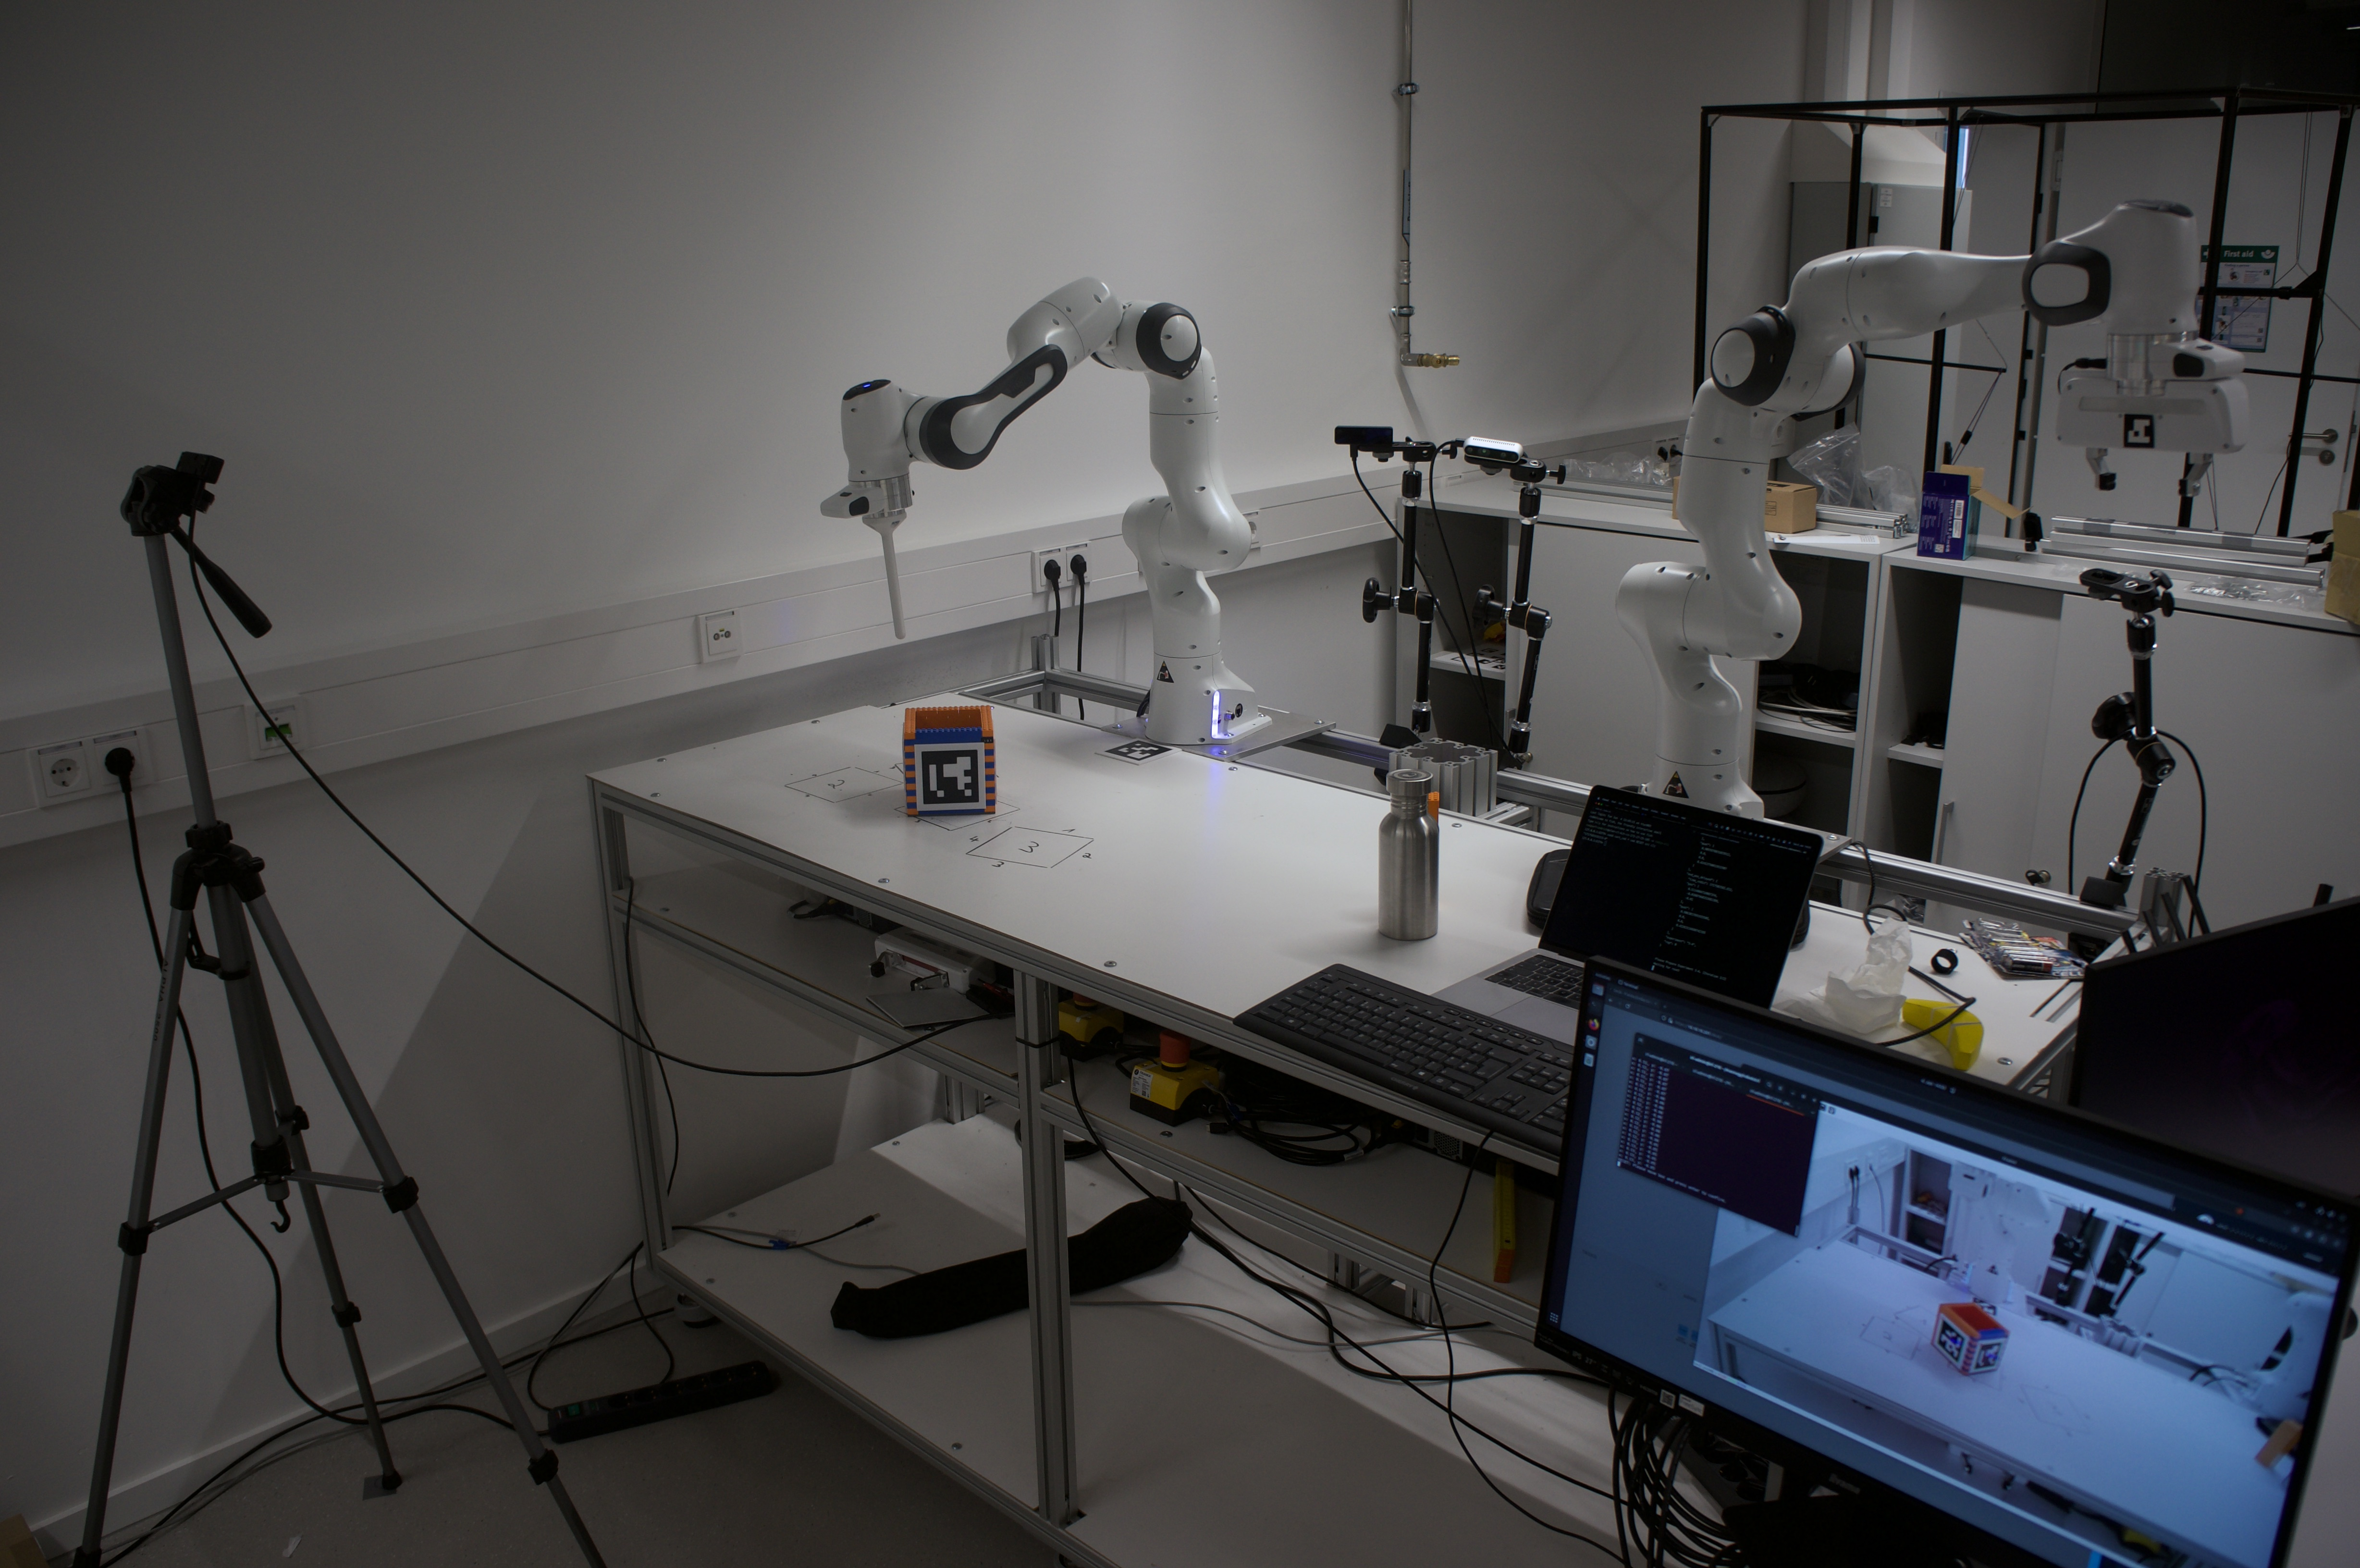
\includegraphics[width=.6\linewidth]{media/labsetup.jpg}

\end{frame}

\begin{frame}
\frametitle{In the Real World}

\begin{columns}[t]
    \begin{column}{0.3\textwidth}
    \end{column}
    \begin{column}{0.5\textwidth}
        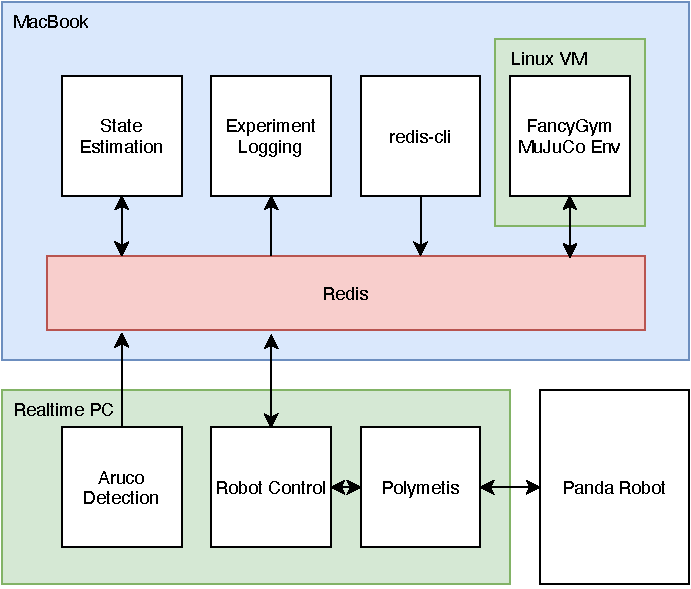
\includegraphics[width=\linewidth]{media/Architecture.pdf}
    \end{column}
\end{columns}
\end{frame}

\begin{frame}
\frametitle{Results}

\begin{columns}[t]
    \begin{column}{0.5\textwidth}
    \end{column}
    \begin{column}{0.5\textwidth}
    \end{column}
\end{columns}
\end{frame}


\appendix
\beginbackup{}
\backupend{}

\end{document}
